% $Id$

In this chapter we review some of the physics underlying the detection of
gravitational waves binary inspiral. Section \ref{s:effect} decribes the
physical effect of a gravitational wave on freely falling test masses and
section \ref{s:ifos} describes how a laser interferometer can be used to
measure this effect. The gravitational waves produced by the inspiral of two
compact objects, such as neutron stars of black holes, are discussed in
section \ref{s:inspiralgw}. We also derive the form of the gravitational
waveform that will be used by the matched filter described in chapter
\ref{ch:findchirp} to extract the gravitational wave signal from
interferometer noise.

\section{The Effect of Gravitational Waves on Freely Falling Particles}
\label{s:effect}

In this section we review the effect of gravitational waves on a pair of
freely falling particles in order to introduce some of the concepts that we
need to discuss the detection of gravitational waves from binary inspirals.
For a detailed decription of the propagation and effect of gravitational
waves, we refer to \cite{MTW73,Thorne:1982cv}. Consider first a single
particle moving in curved spacetime. If the particle is freely falling, its
4-velocity, $\vec{u}$, satisfues the geodessic equation
\begin{equation}
\label{eq:geodessic}
\nabla_{\vec{u}} \vec{u} = \tensor{u}{^\alpha_{;\mu}}u^{\mu} = 0,
\end{equation}
where $;$ denotes the covariant derivative, that is,
\begin{equation}
\tensor{u}{^\alpha_{;\mu}}\tensor{u}{^{\mu}} = \left(\partial_\mu\tensor{u}{^\alpha} +
\Gamma^\alpha_{\mu\nu}u^\nu\right) u^\mu,
\end{equation}
where $\Gamma^\alpha_{\mu\nu}$ is the connection coefficent of the metric
$g_{\alpha\beta}$. Now suppose that we have two particles $A$ and $B$ as shown
in figure \ref{f:particles}. The separation between the particles is
$\vec{\xi}$. The particles are initally at rest with respect to each other, so
\begin{align}
\nabla_{\vec{u}} \vec{u} &= 0, \\
\vec{u} \cdot \vec{\xi} & = 0.
\end{align}
If the spacetime is curved, the second derivative of $\vec{\xi}$ along
$\vec{u}$ is non-zero, however. It is given by the equation of geodessic
deviation
\begin{equation}
\nabla_{\vec{u}}\nabla_{\vec{u}} \vec{\xi} = - R(\_,\vec{u},\vec{\xi},\vec{u})
\end{equation}
where $R(\_,\vec{u},\vec{\xi},\vec{u})$ is the Riemann curvature tensor. We now
introduce a \emph{Local Lorentz Frame} (LLF) for particle $A$. A LLF is
cartesian coordinate system defined by three orthogonally pointing giroscopes
carried by particle $A$. The curvature of spacetime means that the coordinate
system is not exactly cartesian, but it can be shown that this deviation is
second order in the spatial distance from the particle\cite{MTW73}. This means
that along the worldline of particle $A$ the metric is
\begin{equation}
g_{\alpha\beta} = \eta_{\alpha\beta} + \frac{\mathcal{O}\left(|\vec{x}|^2\right)}{R^2}
\end{equation}
where $\eta_{\alpha\beta}$ is the flat Minkowski metric, $\vec{x}$ is the
distance from the particle and $R \sim |R_{\alpha\beta\gamma\delta}|$. In the
Local Lorentz frame of particle $A$, the equation of geodessic deviation
becomes
\begin{equation}
\frac{\partial^2 \xi^{j}}{\partial t^2} = -
\tensor{R}{^j_{\alpha\beta\gamma}}u^\alpha\xi^\beta u^\gamma =
-\tensor{R}{^j_{0k0}} \xi^k
\end{equation}
We assume further that the spacetime is globally flat, so $g_{\alpha\beta} =
\eta_{\alpha\beta}$, with weak gravitational waves propagating in it. We
describe the gravitational waves by $R_{\alpha\beta\gamma\delta}$ which
satisfies the wave equation
\begin{equation}
\eta^{\mu\nu}R_{\alpha\beta\gamma\delta,\mu\nu} = 0.
\end{equation}
What is the effect of these gravitational waves on our test particles $A$ and
$B$? In the Local Lorentz frame, $\vec{\xi}$ is just the coordinates of $B$.
Let the two particles lie on the $x$-axis of the LLF and write
\begin{equation}
\label{eq:bcoords}
\xi^j = x_{(0)}^j + \delta x^j,
\end{equation}
where $x_{(0)}^j$ is the unperterbed location of particle $B$ and $\delta x^j$
is the change is the position of $B$ caused by the gravitational wave.
Substituting equation (\ref{eq:bcoords}) into the equation of geodessic
deviation, we obtain
\begin{equation}
\label{eq:particledev}
\frac{\partial^2 \delta x^j}{\partial t^2} = - \tensor{R}{^j_{0k0}} x_{(0)}^k =
-R_{j0k0} x_{(0)}^k,
\end{equation}
where we have used $\eta_{\alpha\beta}$ to lower the spatial index $j$ of the
Riemann tensor. For a weak gravitational wave, all the components of
$R_{\alpha\beta\gamma\delta}$ are completely determined by $R_{j0k0}$.
Furthermore, it can be shown that the $3\times3$ symmetric matrix $R_{j0k0}$,
which we would expect to have $6$ independent componets, has only $2$
independent components due to the Einstein equations and the Biancci identity.

Let us define the (transverse traceless) gravitational wave field,
$h_{jk}^\mathrm{TT}$, by
\begin{equation}
-\frac{1}{2} \frac{\partial^2 h_{jk}^\mathrm{TT}}{\partial t^2} \equiv
\tensor{R}{_{j0k0}}.
\label{eq:hjkdef}
\end{equation}
Using this definition in equation (\ref{eq:particledev}), we obtain
\begin{equation}
\delta x^j = \frac{1}{2} h_{jk}^\mathrm{TT} x_{(0)}^k.
\end{equation}
If we orient our coordinates so the gravitational waves propagate in the
$z$-direction, so $h_{jk}^\mathrm{TT}(t-z)$, then the only non-zero components
of $h_{jk}^\mathrm{TT}$ are $h_{xx}^\mathrm{TT}$, $h_{yy}^\mathrm{TT}$,
$h_{xy}^\mathrm{TT}$ and $h_{yx}^\mathrm{TT}$. Since $h_{jk}^\mathrm{TT}$ is
transverse and traceless, these components satisfy
\begin{align}
h_{xx}^\mathrm{TT} &= - h_{yy}^\mathrm{TT}, \\
h_{xy}^\mathrm{TT} &= h_{yx}^\mathrm{TT}
\end{align}
and we define the two independent components of the gravitational wave to be
\begin{align}
h_{+} &= h_{xx}^\mathrm{TT} = - h_{yy}^\mathrm{TT}, \\
h_{\times} &= h_{xy}^\mathrm{TT} = h_{yx}^\mathrm{TT}
\end{align}
which we call the \emph{plus} and \emph{cross} polarizations of the
gravitational wave respectively.

Now consider two more particles $C$ and $D$ lying on the $y$-axis of the LLF
separated by 
\begin{equation}
\zeta^j = y^j_{(0)} + \delta y^j
\end{equation}
as shown in figure \ref{f:rings}. A linearly polarized gravitational wave is
one that only contains the plus or the cross polarization. The influence of
a linearly plus polarized gravitational wave propagating in the $z$-direction
is
\begin{align}
\delta x &= \frac{1}{2} h_{xx}^\mathrm{TT} x_{(0)},\\
\delta y &= -\frac{1}{2} h_{yy}^\mathrm{TT} y_{(0)}
\end{align}
and for the and for a linearly $\times$-polarized gravitational wave
propagating in the $z$-direction is
\begin{align}
\delta x &= \frac{1}{2} h_{xy}^\mathrm{TT} y_{(0)},\\
\delta y &= \frac{1}{2} h_{yx}^\mathrm{TT} x_{(0)}.
\end{align}
Figure \ref{f:rings} shows the effect of $h_{+}$ and $h_{\times}$ on a ring
of particles that lie in the $xy$ plane. We can see for the plus polarization
that the that the effect of a gravitational wave is to stretch the particles
in the $x$ direction, while squeezing them in the $y$ direction for the first
half of a cycle and then squeeze in the $x$ direction and stretch in the $y$
direction for latter half of the cycle.  There is therefore a relative change
in length between the two particles $AB$ and $CD$ over the course of a cycle.
For a circularly polarized gravitational wave (which contains both plus and
cross polarizations) propagating in the $z$ direction, $h(t-z) =
h_{+}(t-z) + h_{\times}(t-z)$, the overall effect is
\begin{align}
\delta x &= \frac{1}{2}\left(h_{+}(t-z) x_{(0)} + h_{\times}(t-z) y_{(0)}\right),\\
\delta y &= \frac{1}{2}\left(-h_{+}(t-z) y_{(0)} + h_{\times}(t-z) x_{(0)}\right).
\label{eq:armdisp}
\end{align}
It is this relative change in the lengths of two perpendicular pairs of
particles that we attempt to detect with gravitational wave detectors.We can
see from equation (\ref{eq:armdisp}) that the change in length is proportional
to the original distance between the test masses. For a pair of lest masses
separated by a length $L$, we define the \emph{gravitational wave strain},
$h$, to be the fractional change in length between the masses
\begin{equation}
h = \frac{\Delta L}{L}.
\end{equation}

The lowest order of gravitational radiation is quadrupolar. There is no
``charge'' or ``current'' dipole gravitational ratiation due to conservation
of linear and angular momentum respectively. The amplitude of gravitational
wave strain is that we wish to detect is approximately\cite{thorne.k:1987}
\begin{equation}
h \sim \frac{2G}{c^5} \frac{\partial^2}{\partial t^2} \mathcal{I},
\end{equation}
where $\mathcal{I}$ is the mass quadrupole moment of the source. For typical
astrophysical sources of gravitational radiation that we wish to detect $h
\sim 10^{-22}$. If we separate our test masses by a distance of $4$~km (a
practical distance for Earth bound observatories) the challenge faced by
gravitational wave astronomers is to measure changes of length of order
\begin{equation}
\Delta L \sim 20^{-22} \times 10^4\,\mathrm{m} \sim 10^{-18}\,\mathrm{m}.
\end{equation}

\section{The LIGO Gravitational Wave Detectors}
\label{s:ifos}

As described above, in order to detect gravitational waves, we must measure
the change in distance between freely falling test masses. There are several
major efforts underway\cite{Barish:1999,Acernese:2002,Luck:1997hv} to measure
the strain produced by a gravitational wave using \emph{laser
interferometery}. In this thesis we analyze data from the Laser Interferometer
Gravitational wave Observatory, LIGO. LIGO operates three
\emph{power-recycled-Fabry-Perot-Michelson} interferometers in the United
States, shown in figure \ref{f:usmap}. Two of these are colocated at the LIGO
Hanford Observatory, WA (LHO) and one at the LIGO Livingston Observatory
(LLO). The interferometers at the LHO are 4~km and 2~km in arm length and are
refered to as H1 and H2, respectively. The interferometer at the LLO is a 4~km
long interferometer refered to as L1.  In this section we consider the
essential design features of these interferometer that allow them to be
sensitive astrophysical gravitational wave sources.

\subsection{The Design of the LIGO Interferometers}
\label{ss:ligoifos}

Interferometric gravitational wave detectors use laser light to measure the
change in postion of ``freely falling'' test masses\footnote{The
test masses in an Earth bound gravitational wave observatory are not truely
freely falling as they are accellerated, but we ignore this effect here as it 
is unimportant. See for example \ref{Thorne:1982cv} for a full treatment of
the effect of gravitational waves on an Earth bound interferometer}, i.e. the
mirrors of the interferometer.  The challenge facing experimenters
constructing a gravitational wave interferometer is to measure changes of
length of order $\sim 10^{-18}\,\mathrm{m}$ using laser light has a wavelength
of $\lambda_l \sim 10^{-6}$~m.  It should be noted that measuring a phase
shift of
\begin{equation}
\Delta \Phi \sim \frac{\Delta L}{\lambda_l} \sim 10^{-12}
\end{equation}
is a factor $10^{12}$ more sensitive than the interferometers used by
Michelson and Morely to disprove the existance of the ether.

The basic concept is of a gravitational wave interferometer is illustrated in
figure \ref{f:ifodesign} (a). Such a configuration is refed to as a
\emph{simple Michelson} interferometer. Laser light is shone on a \emph{beam
splitter} which reflects half the light in to the \emph{$x$-arm} and transmits
half the light into the \emph{$y$-arm} of the interferometer. The light
travels a distance $L$ in each arm and then is reflected back towards the beam
splitter by the \emph{end test masses}. Consider the light in the $x$-arm. The
space-time interval between the beam splitter and the end test mass is given
by
\begin{equation}
ds^2 = g_{\mu\nu}\, dx^\mu\, dx^\nu = 0.
\label{eq:dist}
\end{equation}
The metric of spacetime in the presence of a weak gravitational wave is
\begin{equation}
g_{\mu\nu} = \eta_{\mu\nu} + h_{\mu\nu},
\end{equation}
where all the components of $h_{\mu\nu}$ are zero, appart from those defined
in equation (\ref{eq:hjkdef}). In the presence of a plus polarized,
sinusoidal, gravitational wave travelling in the $z$-direction, equation
(\ref{eq:dist}) becomes
\begin{equation}
c^2 dt^2 = \left(1 + h_{+}(t-z)\right) dx^2 + \left(1 - h_{+}(t-z)\right) dx^2,
\end{equation}
We can measure the response of the interferometer to a gravitational wave by
considering the phase shift of light in the arms. The phase that the light
aquires propagating between the beam splitter to the $x$-end test mass and
back is is given by\cite{Saulson:1994}
\begin{equation}
\begin{split}
\Phi_x &= \int_0^{\tau_\mathrm{RT}} 2\pi f_l\, dt \\
&= \frac{1}{c} \int_0^L 2\pi f_l \sqrt{1 + h_{+}}\,dx -
\frac{1}{c} \int_L^0 2\pi f_l \sqrt{1 + h_{+}}\,dx \\
&\approx \frac{2\pi f_l L}{c} \left(1 + \frac{h_{+}}{2}\right),
\end{split}
\end{equation}
where $\tau_\mathrm{RT}$ is the round trip proper time of the light and $f_l$ is
its frequency. We have discareded  higher order terms in $h_+$ as they are
negligable.  We can see that the phase shift aquired in the $x$-arm due to the
gravitational wave is
\begin{equation}
\delta \Phi_x = \frac{2\pi}{\lambda_l} h_{+} L.
\end{equation}
A similar calulation shows that the phase shift aquired in the $y$-arm is
\begin{equation}
\delta \Phi_y = - \frac{2\pi}{\lambda_l} h_{+} L
\end{equation}
and so the difference in phase shift between the arms is
\begin{equation}
\Delta \Phi = \frac{4\pi}{\lambda_l} h_{+} L.
\end{equation}
A typical astrophysical source of gravitational radiation of interest to LIGO,
has a frequency $f_\mathrm{GW} \sim 100$~Hz. Therefore the wavelength of the
gravitational wave is $\lambda_\mathrm{GW} \sim 3000$~km. Notice that if
$\tau_\mathrm{RT} = 1 / f_\mathrm{GW}$ there will be no phase shift of the
light. The light spends exactly one gravitational wave period in the arm and
so the phase shift aquired by positive values of $h_+(t-z)$ is cancelled out
by the phase shift due to negative values of $h_+(t-z)$. The interferometer
achives maximum sensitvity when the light spends half a gravitational wave
period in the arms, that is
\begin{equation}
L = \frac{\lambda_\mathrm{GW}}{2} \sim 1000\,\mathrm{km}.
\end{equation}
This is hopelessly impractical for a Earth bound detector. In order to solve
this problem, we enhance our simple Michelson interferometer by cing two
additional mirrors in the arms of the interferometer, known as the inner $x$
and $y$ test masses, as shown in figure \ref{f:ifodesign} (b). The aim of
these mirrors is to bounce the light in the arms for approximately one half of
a gravitational wave period.  The mirrors create a \emph{Fabry-Perot cavity}
in the arms which store the light for $B \sim 200$ bounces, increasing the
phase shift by a factor of $B$
\begin{equation}
\Delta \Phi = 4\pi \frac{L}{\lambda_l} h_{+} \sim 
10 \cdot \frac{4 \times 10^3\,\mathrm{m}}{10^{-6}\,\mathrm{m}} \cdot 200 \cdot
10^{-21} \sim 10^{-9}.
\end{equation}
This gains us 3 orders of magnitude above of initial estimate of $10^{-12}$.
Increasing $B$ does not gain any sensitivity, however, as phase storing the
light for longer than half a gravitational wave period causes it to lose phase
shift as as the sign of the gravitational wave changes.

Is it possible to measure a phase shift of $10^{-9}$ using a
Fabry-Perot-Michelson interferometer? We measure the phase shift by averaging
the light at the photodiode over some period, $\tau$. Let $N$ be the number of
photons from the laser arriving at the photodiode in the time $\tau$. The
measured number of photons in the averaging interval is a Poisson process,
with probability distribution function for $N$ given by
\begin{equation}
p(N) = \frac{ \bar{N} ^{N} \exp \left(-\bar{N}\right) } {N!},
\end{equation}
where $\bar{N}$ is the mean number of photons per interval $\tau$. A very
large number of photons, $N_\gamma \gg 1$, will arrive at the photodetector in
the averaging time, however, so this Poisson distribution can be approximated
by a Gaussian distribution. The uncertainty in the number of photons arriving in the
averaging time is therefore
\begin{equation}
\Delta N = \sqrt{N}.
\end{equation}
The accuracy that we can measure the phase shift for a given amount of input
laser power is constrained by the uncertainty principle,
\begin{equation}
\Delta t \, \Delta E \ge \hbar.
\label{eq:uncertainty}
\end{equation}
The energy the light arriving at the photodiode in time $\tau$ is
\begin{equation}
E = \hbar \frac{2\pi c}{\lambda_l} N
\end{equation}
which, due to the counting of photons, has uncertainty 
\begin{equation}
\Delta E = \hbar \frac{2\pi c}{\lambda_l} \sqrt{N}.
\label{eq:uncertdeltae}
\end{equation}
Using this and $\Delta\Phi = 2\pi c \Delta t / \lambda_l$ and the uncertainty
principle, equation (\ref{eq:uncertainty}), we obtain
\begin{equation}
\Delta t \, \Delta E = \frac{\Delta \Phi \lambda_l}{2\pi c} \hbar \frac{2\pi
c}{\lambda_l} N \ge \hbar
\end{equation}
and so the accuracy which which we can measure the phase is no better than
\begin{equation}
\Delta \Phi \ge \frac{1}{\sqrt{N}}.
\end{equation}
This equation tells us how many photons we need in an averaging period to
measure a given phase shift. The optimal averaging time for a gravitational
wave with freqency $f_\mathrm{GW}$ is half a period, that is
\begin{equation}
\tau \approx \frac{1}{2 f_\mathrm{GW}}.
\end{equation}
The intensity of laser light required to measure a phase shift of $10^{-9}$
for a gravitational wave of $f_\mathrm{GW} \sim 100$~Hz is then
\begin{equation}
\begin{split}
I &= N \frac{2 \pi \hbar c \cdot 2f_\mathrm{GW}}{\lambda_l} \\
&\sim \left(\frac{1}{10^{-9}}\right)^2 
\frac{10^2 \times 10^{-34} \times 10^{8} 10^2 } { 10^{-6} } \sim 10^2\,
\mathrm{W}.
\end{split}
\end{equation}
Lasers used in the first generation of interferometers have a typical output
power of $\sim 5$~W. The final enhacement we make to the Michelson
intereferometer is a \emph{power recycling mirror} place between the beam
splitter and the laser, as shown in figure \ref{f:ifodesign} (c). This reflects
some of the laser light back into the interferometer and increases the power
incident on the photodiode so that the phase shift due to a gravitational wave
of order $h \sim 10^{-21}$ can be measured.

The lengths of the arms must be maintained at an integral number of
wavelengths of the light so that the phase shift of light in the two arms
cancells in the absence of a gravitational wave. The power recycling and
Fabry-Perot cavites must also be kept in resonance, so the required power
build up in these cavities are achived. This requires a complicated
\emph{length sensing and control system}\cite{sigg} which continuously
monitors the position of the mirrors in the interferometer and sends feedback
motions via electromagnetic actuators to keep the interferometer
\emph{locked}. The optics and control loop form the core systems of the
interferometer, however there are many subtleties to the design and operation
of a gravitataional wave interferometer this which are outside the scope of
this thesis.

\subsection{Noise sources in an Interferometer}
\label{ss:noise}

A gravitational wave in the interferometer would produce a signal 
\begin{equation}
h(t) = \frac{\Delta L_x - \Delta L_y}{L}
\end{equation}
in the interferometer, however, there are many sources of noise that are added
to the measured signal in addition to the signal.  Noise sources reduce the
sensitivity of the interferometer to grvaitational waves. The primary goal of
the experimenters engaged in comissioning the detectors is the reduction of
noise in the detector and remarkable progress has been made in increasing the
sensitiving of the LIGO detectors.  For a detailed review of the noise sources
present in kilometer scale interferometer, we refer the reader to
\cite{rana:thesis}. The noise in interferometers is often measured as the
\emph{amplitude spectral density}, $\tilde{h}(f) / \sqrt{\mathrm{Hz}}$. This
is the square root of the power spectral density of the gravitational wave
strain measured by the detector.  Figure \ref{f:design_noisecurve} shows noise
spectral density of the initial LIGO detectors. There are three
``fundamental'' noise sources that limit the sensitivity of the LIGO
detectors; noise sources built into the design of the initial LIGO
interferometer which limit its ultimate sensitivity.  Two of these sources are
known as \emph{displacement noise} and one is known as \emph{sensing noise}.
Displacement noise directly moves the mirrors and causes so causes a
differential change in the lengths of the arms.  Sensing noise is signal that
appears in the output of the gravitational wave detector, but is not due to
motion of the mirrors.  The three noise sources shown in figure
\ref{f:design_noisecurve} are
\begin{enumerate}
\item \emph{Seismic noise.} This is the domainant noise at low frequencies, $f
\lesssim 40$~Hz.  Seiesmic motion of the earth couples through the suspension
of the mirror and causes it to move. To mitigate this, a system of coupled
oscillators is used to isolate the mirror from the ground motion. 

\item \emph{Suspension thermal noise.} This noise source limits the
sensitvity of the interferometer in the range $40$~Hz~$\lesssim f \lesssim
200$~Hz. The steel wire suspening the mirror is at room temperature and
thermal motion of the particles in the wire produce motion of the mirror and
change the arm length.

\item \emph{Photon shot noise.} At high frequencies, $f \gtrsim 200$~Hz, the
noise is dominated by the shot noise due to the photon counting statistics
discussed in the precious section.
\end{enumerate}

\subsection{Calibration of the Data}
\label{ss:calibration}

The output of the interferometer is not actually a gravitational wave strain.
The signal recorded to disk is the error signal of the feedback loop used to
control the differntial lengths of the arms. This signal is known as
\texttt{LSC-AS\_Q} and contains the gravitational wave signal.  In this
thesis, we refer to the error signal as $v(t)$.  The gravitational wave signal
can be reconstructed from the error signal in the frequency domain by the
\emph{response function}, $R(f)$, of the instrument by
\begin{equation}
\tilde{h}(f) = R(f) \tilde{v}(f).
\end{equation}
The response function is constructed from three elements of the feedback loop:
a sensing function, $C(f)$, an actuation function, $A(f)$, and a digital
feedback filter, $D(f)$\cite{gaby}. 

The sensing function $C(f)$ measures the response of the response of the arm
cavities to gravitational waves. It is dependent on the power in the arm,
which changes over time as the alignment of the mirrors change.  The actuation
function, $A(f)$, is the response of the mirrors to the electromagnets used to
control the length of the cavities. The major contribution to this is the
pendulum response of the suspended mirrors.  The digital filter, $D(f)$, is
the feedback control system that converts the error signal, $v(t)$, into a
control signal that is sent as actuation to the mirrors to keep the cavities
resonant.

We describe the closed feedback loop of the interferometer as follows. The
\emph{residual length}, $r(f)$, of the differential mode cavity is the sum of
the strain in the arms, $s(f) = h(f) + n(f)$, (which may be due to
gravitational waves, $h$ and noise, $n$) and the effect of the control signal,
$g$, applied to the mirror
\begin{equation}
r(f) = s(f) - A(f)g(f).
\end{equation}
This net strain produces an error signal given by sensing function
\begin{equation}
v(f) = C(f) r(f)
\end{equation}
end this error signal is converted into a control signal by the digital filter 
\begin{equation}
g(f) = D(f) v(f) = D(f) C(f) r(f),
\end{equation}
which in turn is fed back into the mirrors. The residual length is therefore
\begin{equation}
r(f) = s(f) - A(f)D(f)C(f) r(f)
\end{equation}
which can be written as
\begin{equation}
r(f) = \frac{s(f)}{1 + A(f)D(f)C(f)} = \frac{s(f)}{1 + G(f)},
\end{equation}
where $G(f)$ is the \emph{open loop gain} of the interferometer, defined by
$G(f) = A(f)D(f)C(f)$. The measured signal is then
\begin{equation}
v(f) = C(f) r(f) = s(f) \frac{C(f)}{1 + G(f)}
\end{equation}
and we see that the response function, $R(f)$, used to calibrate the signal is
given by
\begin{equation}
R(f) = \frac{1 + G(f)}{C(f)}.
\end{equation}

The value of the digital filter, $D(f)$ is a known function of time since it
the algorithm used to control the lengths of the cavities.  The actuation
function can be measured by configuring the interferometer as a simple
Michelson, driving a mirror and counting the number of fringes that appear at
the photodide for a given applied signal. Since $A(f)$ is a due to the
pendulum response of the mirror and filters using in the electronics that
drive the motion of the mirror, it does not change and its value can be
established before data taking. Once the displacement of the mirror in
response to an applied control signal is known (refered to as the DC gain), a
sinusoidal signal of known amplitude that sweeps up in freqency is added to
the control signal. By comparing the amplitude of the \emph{calibration sweep}
in the output of the detector to the known input, the value of the open loop
gain and (and hence the sensin function) can be determined. The values of the
sensing function and open loop gain at the time of calibration are denoted
$C_0(f)$ and $G_0(f)$.

The LIGO detectors have an alignment control system that tries to keep the
power in the arms constant, however the power in the cavity can still change
significantly over the course of data taking. This fluctuation in power means
that the sensing function can change on time scales of order minutes or hours.
To measure $C(f)$ during data taking, \emph{calibraion lines} are injected
into the interferometer. These are sinusoidal signals of known amplitude and
frequency, $f_\mathrm{cal}$, added to the control signals that drive the
mirrors.  By measuring the amplitude of the calibration line over the course
of the run compared to the time at which the calibration sweep was taken, we
may measure the change in the sensing function
\begin{equation}
C(f;t) = \alpha(t) C_0(f),
\end{equation}
where $\alpha(t)$ is the ratio of the calibration line amplitide at time $t$
to the reference time. We also allow the digital gain of the feedback loop to
vary by a known factor, $\beta(t)$. The response function at any given time,
$t$, becomes
\begin{equation}
R(f;t) = \frac{1 + \alpha(t)\beta(t)G_0(f)}{\alpha(t)C_0(f)}.
\end{equation}

\section{Gravitational Waves from Binary Inspiral}
\label{s:inspiralgw}

\subsection{The post$^2$-Newtonian Waveform}

\subsection{The Stationary Phase Approximation}
\label{ss:stationaryphase}

The inspiral waveforms that we need in the matched filter are $\tilde{h}_c(f)$
and $\tilde{h}_s(f)$, rather than the waveforms $h_c(t)$ and $h_t(t)$ computed
in chapter \ref{ch:inspiral}. There are two ways of obtaining $\tilde{h_c}(f)$.
The first is to compute $h_c(t)$ then Fourier transform the signal. This is
compulationally expensive, however, as it requires an additional FFT for each
template that we wish to filter. The second method is to use the stationary phase
approximation\cite{Mathews:1992} to express the chirp directly in the frequency
domain\cite{WillWiseman:1996,Cutler:1994}. Given a function
\begin{equation}
B(t) = A(t) \cos \phi(t)
\end{equation}
where
\begin{equation}
\frac{d\ln A}{dt} \ll \frac{d\phi}{dt}
\end{equation}
and
\begin{equation}
\frac{d^2\ln A}{dt^2} \ll \left(\frac{d\phi}{dt}\right)^2
\end{equation}
then the stationary phase approximation to the Fourier transform of $B(t)$ is
given by
\begin{equation}
\tilde{B}(f) = \frac{1}{2} A(t) \left(\frac{df}{dt}\right)^{-\frac{1}{2}}
\exp\left[ -i \left(2\pi f t' - \phi(f) - \frac{\pi}{4} \right)\right]
\end{equation}
where $t'$ is the time at which
\begin{equation}
\frac{d\phi(t)}{dt} = 2\pi f
\end{equation}
and
\begin{equation}
\phi(f) = \phi\left[t(f)\right].
\end{equation}

For the restricted post$^2$-Newtonian chirps discussed in chapter
\ref{ch:inspiral}, the orbital frequency at any instant is given by
\begin{equation}
\Omega = \frac{M^{\frac{1}{2}}}{r^{\frac{3}{2}}}.
\end{equation}
The inspiral rate for circular orbits is given by
\begin{equation}
\frac{dr}{dt} = - \frac{r}{E} \frac{dE}{dt} = 
- \frac{64}{5} \frac{\mu M^2}{r^3}.
\end{equation}
Thus
\begin{align}
r^3 \, dr &= - \frac{64}{5} \mu M^2 \, dt \\
\frac{r^4}{4} &= \frac{64}{5} \mu M^2 (t - t_c)
\end{align}
and so
\begin{equation}
r(t) = \left(\frac{256}{5} \mu M^2 \right)^{\frac{1}{4}}
       \left(t_c - t\right)^{\frac{1}{4}}.
\end{equation}
Since the emitted radiation is quadrupolar
\begin{equation}
f = \frac{\Omega}{\pi}.
\end{equation}
The gravitational wave strain is
\begin{equation}
h(t) = \frac{Q}{D} \left(\frac{384}{5}\right)^\frac{1}{2} \pi^\frac{2}{3} \mu M
r^{-1}(t) \cos \left( \int 2\pi f(t) \, dt \right).
\end{equation}
Now
\begin{align}
\frac{df}{dt} 
     &= \frac{d}{dt} \left(\frac{\Omega}{\pi}\right) 
      = \frac{d}{dt} \left(\frac{M^\frac{1}{2}}{\pi} r^{-\frac{3}{2}}\right) \\
     &= \frac{M^\frac{1}{2}}{\pi} \frac{dr}{dt} \left(-\frac{3}{2} r^{-frac{5}{2}}\right) \\
     &= \frac{M^\frac{1}{2}}{\pi} \left(-\frac{64}{5} \frac{\mu M^2}{r^3}\right)
        \left(-\frac{3}{2} r^{-frac{5}{2}}\right) \\
     &= \frac{96}{5} \frac{M^\frac{5}{2} \mu}{\pi} r^{-\frac{11}{2}}. 
     \label{eq:sp:dfdt}
\end{align}
Now
\begin{equation}
f = \frac{M^\frac{1}{2}}{\pi} r^{-\frac{3}{2}}.
\end{equation}
Solving this for $r$, we obtain
\begin{equation}
r = \frac{M^\frac{1}{3}}{\pi^\frac{2}{3} f^\frac{2}{3}}
\end{equation}
which we can substitute into equation (\ref{eq:sp:dfdt}) and obtain
\begin{align}
\frac{df}{dt} &= \frac{96}{5} \pi^\frac{8}{3} \mu M^\frac{2}{3} f^\frac{11}{3} \\
&= \frac{96}{5} \pi^\frac{8}{3} \mathcal{M}^\frac{5}{3} f^\frac{11}{3}
\end{align}
where we have defined the \emph{chirp mass} by
\begin{equation}
\mathcal{M} = \mu^\frac{3}{5} M^\frac{2}{5}.
\end{equation}
Now the phase is given to post$^2$-Newtonian order by\cite{Blanchet:1996pi}
\begin{equation}
\phi(t) = \int^t 2\pi f(t') \, dt'
\end{equation}
we won't worry about this yet.

Therefore using the stationary phase approximation, we obtain
\begin{align}
\tilde{h}(f) &= \frac{1}{2} \frac{Q}{D} \left(\frac{384}{5}\right)^\frac{1}{2} \pi^{2}{3} \mu M
                r^{-1}(t) \left(\frac{df}{dt}\right)^{-\frac{1}{2}} \exp\left[-i \Psi\right] \\
             &= \frac{1}{2} \frac{Q}{D} \left(\frac{384}{5}\right)^\frac{1}{2} \pi^{2}{3} \mu M
                \frac{\pi^\frac{2}{3} f^\frac{2}{3}}{M^\frac{1}{3}}
                \left(\frac{df}{dt}\right)^{-\frac{1}{2}} \exp\left[-i \Psi\right] \\
             &= \frac{1}{2} \frac{Q}{D} \left(\frac{384}{5}\right)^\frac{1}{2} \pi^{4}{3} \mu
                M^\frac{2}{3} r^\frac{2}{3}
                \left(\frac{df}{dt}\right)^{-\frac{1}{2}} \exp\left[-i \Psi\right].
\end{align}
Now
\begin{equation}
\left(\frac{df}{dt}\right)^{-\frac{1}{2}} =
\left(\frac{5}{96}\right)^\frac{1}{2} \pi^{-\frac{4}{3}} 
\mu^{-\frac{1}{2}} M^{-\frac{1}{3}} f^{-\frac{11}{6}}
\end{equation}
and so 
\begin{align}
\tilde{h}(f) &= \frac{1}{2} \frac{Q}{D} \left(\frac{384}{5} \frac{5}{96}\right)^\frac{1}{2}
                \mu^\frac{1}{2} M^\frac{1}{3} f^{-\frac{7}{6}} \exp\left[-i \psi\right] \\
             &= \frac{Q}{D} \mathcal{M}^\frac{5}{6} f^{-\frac{7}{6}} \exp\left[-i \psi\right].
             \label{eq:sp:template}
\end{align}
Equation (\ref{eq:sp:template}) is the stationary phase binary inspiral
template that we will use in the matched filter.

Discussion of validity of SP waveform.

\begin{equation}
t = \frac{5m}{256\eta} 
  x^{-8}\left(1 + \alpha x^2 + \beta x^3 + \gamma x^4 \right)
 \label{eq:chirplength}
\end{equation}
where
\begin{eqnarray}
x & = & \left(\pi m T_\odot f_{\mathrm{low}}\right)^{\frac{1}{3}}, \\
\alpha & = & \frac{743}{252} + \frac{11}{3}\eta, \\
\beta & = & -\frac{32\pi}{3}, \\
\gamma & = & \frac{3058673}{508032}+\frac{5429}{504}\eta+\frac{617}{71}\eta^2,
\end{eqnarray}
$m$ is the mass of the more massive object and $f_{\mathrm{low}}$ is the low
frequency cutoff of the inspiral template.

\newpage

\begin{figure}[p]
\begin{center}
%\includegraphics[width=\linewidth]{figures/inspiral/}
A picture of the worldline of a pair of particles separated by $\xi$.
\end{center}
\caption{\label{f:particles}%
A picture of the worldline of a pair of particles separated by $\xi$.
}
\end{figure}

\begin{figure}[p]
\begin{center}
%\includegraphics[width=\linewidth]{figures/inspiral/}
The standard picture of wibbling rings.
\end{center}
\caption{\label{f:rings}%
The standard picture of wibbling rings.
}
\end{figure}

\begin{figure}[p]
\begin{center}
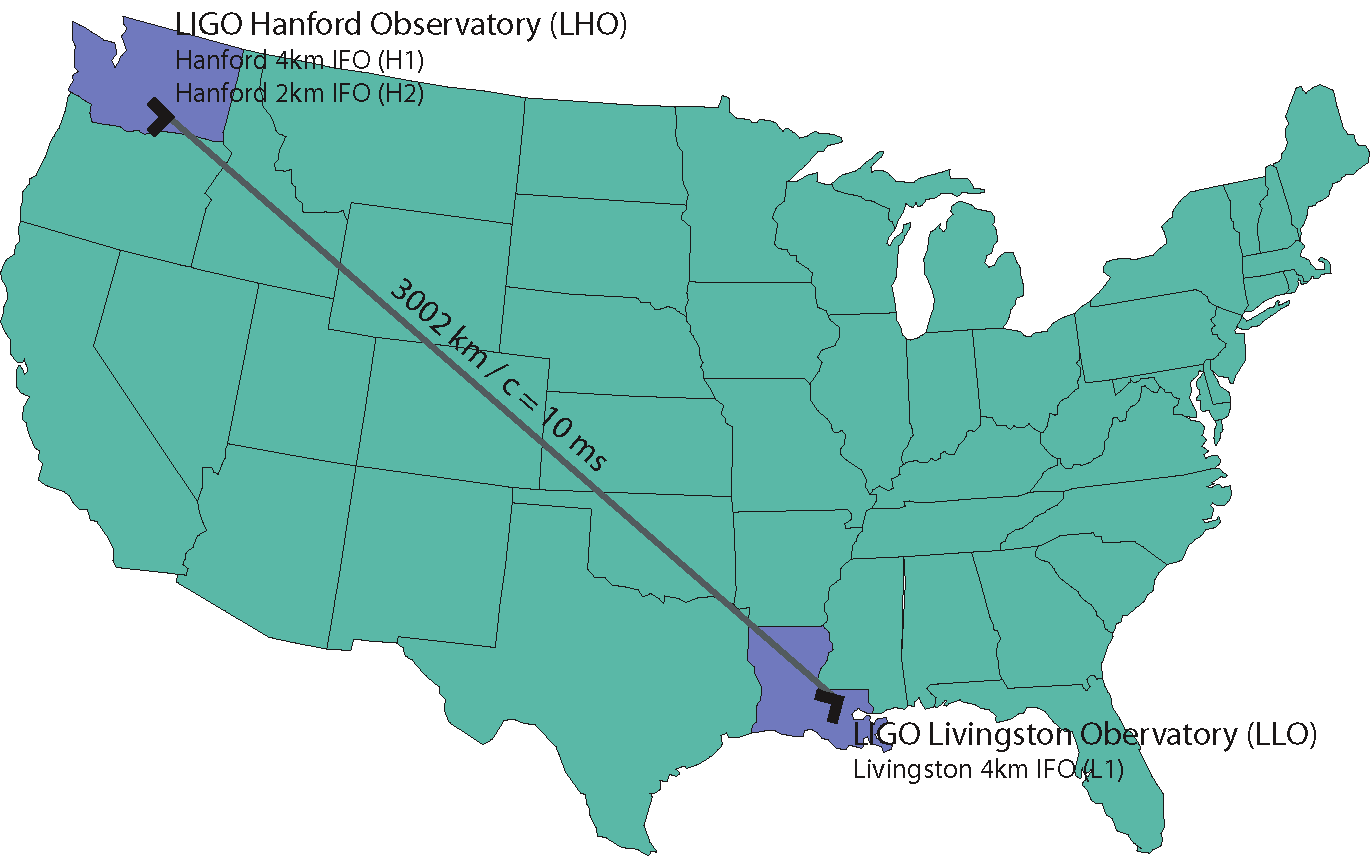
\includegraphics[width=\linewidth]{figures/inspiral/observatories}
\end{center}
\caption{\label{f:usmap}%
The location of the two LIGO observatories.
}
\end{figure}

\begin{figure}[p]
\begin{center}
%\includegraphics[width=\linewidth]{figures/inspiral/}
Here's some pictures of IFO configurations.
\end{center}
\caption{\label{f:ifodesign}%
Here's some pictures of IFO configurations.
}
\end{figure}

\begin{figure}[p]
\begin{center}
%\includegraphics[width=\linewidth]{figures/inspiral/}
The fundamental noise sources of Initial LIGO.
\end{center}
\caption{\label{f:design_noisecurve}%
The fundamental noise sources of Initial LIGO.
}
\end{figure}
